\begin{figure}\label{fig:eval-cost}
  \centering
    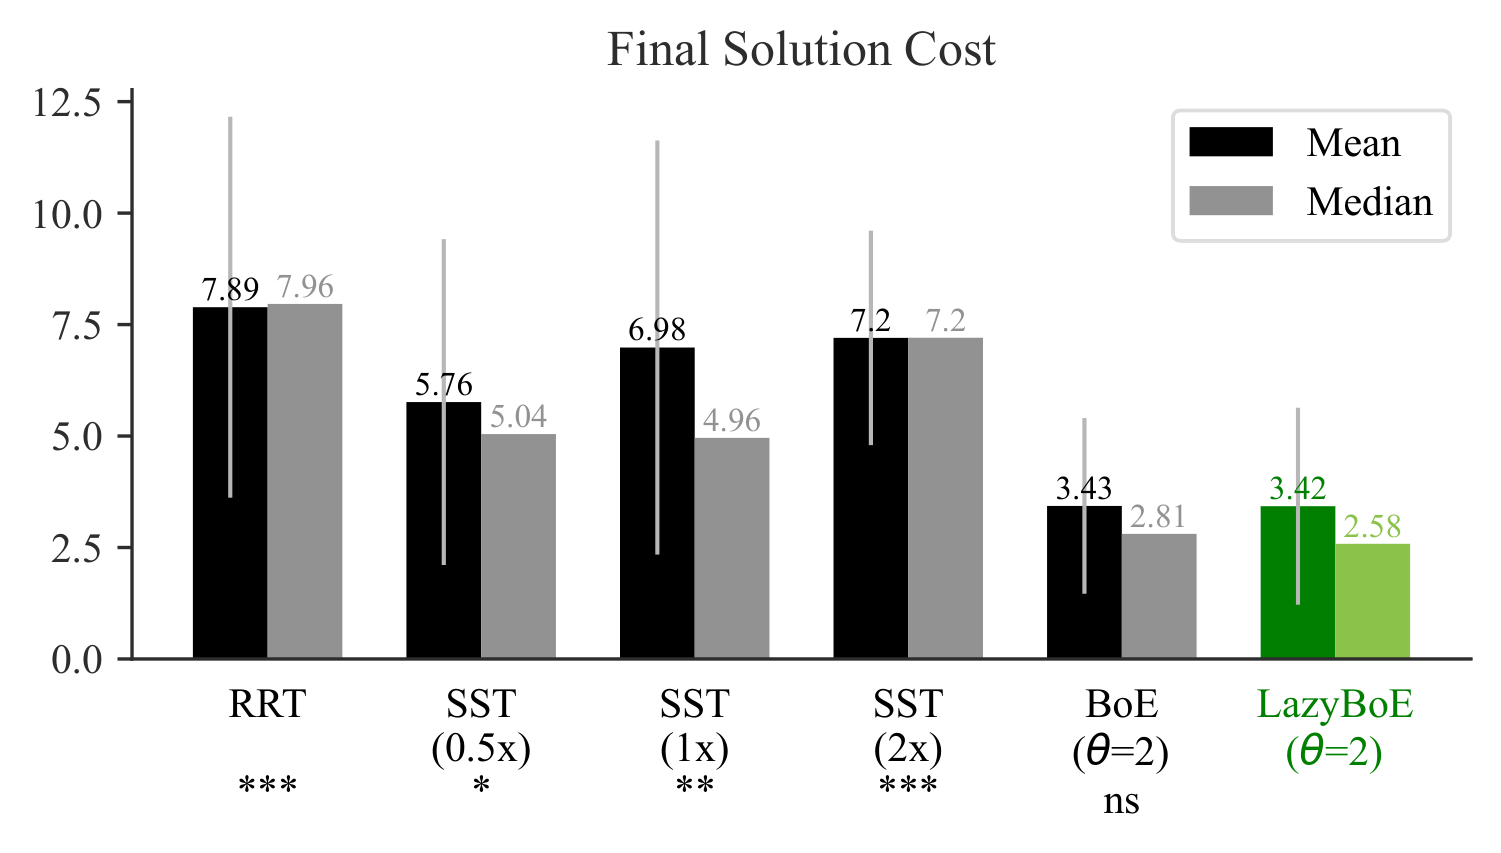
\includegraphics[width=\columnwidth]{assets/final_traj_cost.png}
  \caption{The final solution cost, i.e., the solution with the lowest cost, for our planner is comparable to the BoE planner. Asterisks indicate significance levels.}\label{fig:eval-cost}
\end{figure}
\begin{figure}\label{fig:eval-num_solutions}
  \centering
    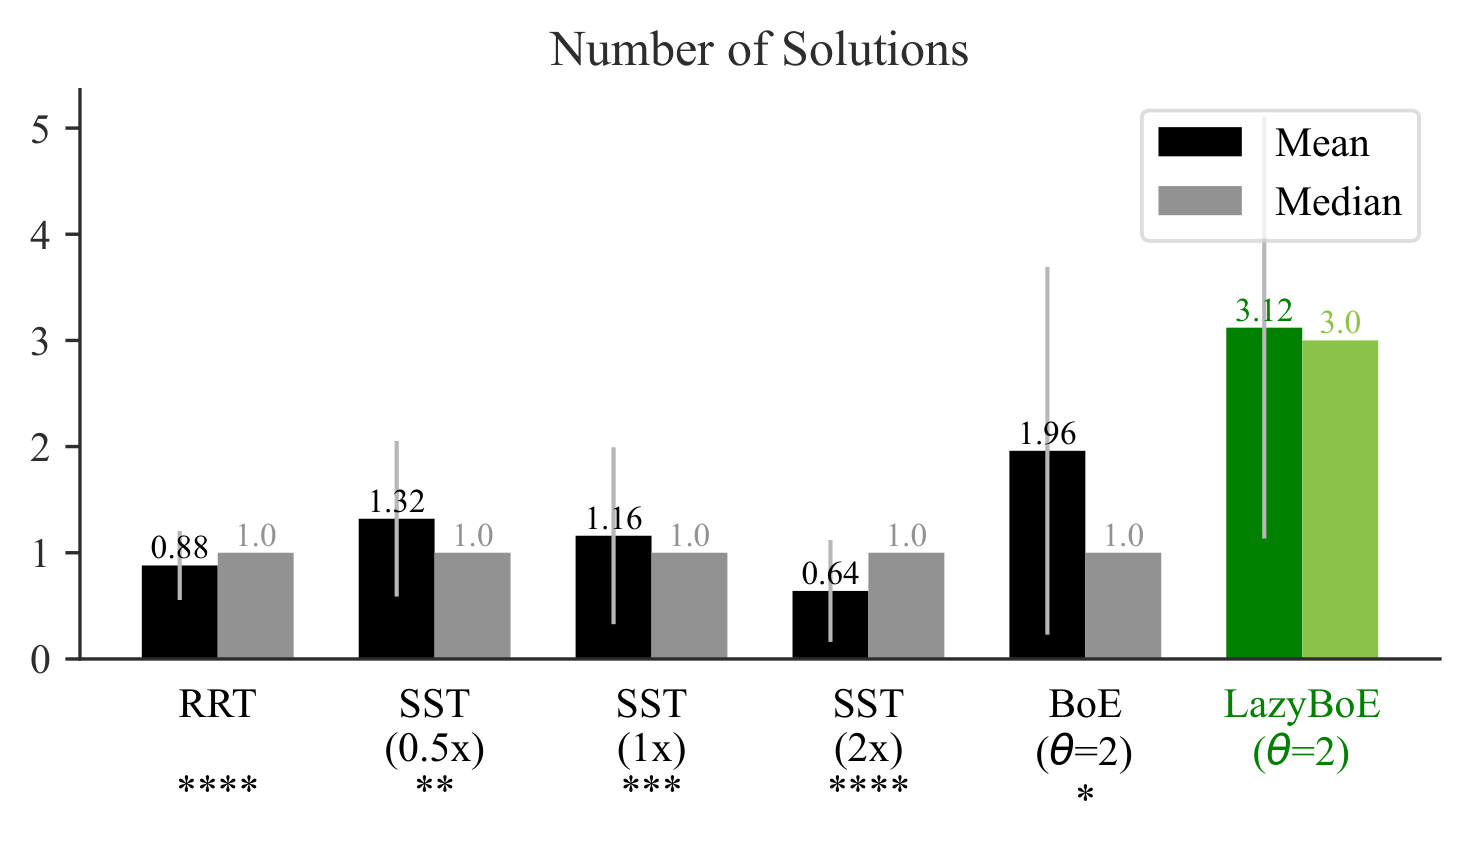
\includegraphics[width=\columnwidth]{assets/num_solutions.png}
  \caption{Our planner is able to explore a larger number of solutions than the baseline methods. RRT terminates after finding the first solution, but the mean number of solutions is less than $1$ because RRT does not succeed in finding a solution for every planning problem \cref{fig:eval-success}. Asterisks indicate the significance levels.\vspace{-10pt}}\label{fig:eval-num_solutions}
\end{figure}

\subsection{Significance Testing}

Statistical analysis using the Mann-Whitney U test further reinforces the results above.
$p-$values for each test are highlighted in \cref{fig:eval-time}, \cref{fig:eval-cost}, and \cref{fig:eval-num_solutions} and marked by `ns' for $p > 0.05$, `*' for $p \leq 0.05$, `**' for $p \leq 0.01$, `***' for $p \leq 0.001$, and `****' for $p \leq 0.0001$.

\textsl{LazyBoE}'s speedup improvement is statistically significant with respect to most baseline algorithms, with notably low $p-$values in comparison to RRT, SST ($0.5$x), and SST ($2$x). However, the comparison with SST ($1$x) did not reach statistical significance (p = 0.0529), indicating that the time difference with this baseline is not conclusive.

For a more robust analysis, we look at the median value, which provides a more accurate representation of the data's central tendency, particularly in the presence of a skewed distribution.
\textsl{LazyBoE} has a lower median cost when compared to various iterations of SST (0.5x) and RRT, demonstrating a potential advantage. It is worth noting that the cost comparison with the BoE algorithm did not yield a significant difference (p = 0.8142), suggesting comparable cost-efficiency between these two algorithms.
Our algorithm also generated a higher median number of solutions compared to all baselines, with statistically significant results in all comparisons.
In summary, this significance testing reinforces our claims that \textsl{LazyBoE} offers performance improvements in terms of both speed and cost-effectiveness.
